\documentclass[conference]{IEEEtran}
\usepackage{amsmath,amssymb}
\usepackage{graphicx}
\usepackage{booktabs}
\usepackage{array}
\usepackage{cite}
\usepackage{listings}
\usepackage{xcolor}
\usepackage{tikz}
\usetikzlibrary{shapes.geometric,arrows.meta,positioning,automata,calc}
\usepackage[hidelinks]{hyperref}

\lstset{basicstyle=\ttfamily\scriptsize,breaklines=true,frame=single,
  keywordstyle=\color{blue!60!black},commentstyle=\color{green!40!black},
  language=Python,columns=fullflexible,xleftmargin=2pt,xrightmargin=2pt,
  showstringspaces=false,morekeywords={yield}}

\newcommand{\pax}{\textit{pax}}
\hyphenation{sched-ul-ing}

\begin{document}
\title{Modeling, Simulation and Scheduling Optimization of the MUET Point (Bus) System Using Queuing Theory and Discrete Event Simulation}

\author{\IEEEauthorblockN{Muhammad Uzair (22SW106)}
\IEEEauthorblockA{Department of Software Engineering\\
Mehran University of Engineering and Technology, Jamshoro, Pakistan\\
PBL Assignment -- Modeling and Simulation}}

\maketitle

\begin{abstract}
Mehran University of Engineering and Technology (MUET) moves thousands of students and staff every day with a fixed fleet of buses (``Points'') between Hyderabad and Jamshoro. During the 08:00--09:00 and 14:00--15:30 peaks the STC and Main Gate terminals suffer long waits because the static timetable cannot follow demand. This report models the system as a time-varying multi-server queueing network, implements it as a discrete event simulation (DES) in Python/SimPy, and compares four scheduling policies on the \emph{existing} fleet of 12 buses: a static baseline (P0), a peak-aware timetable (P1), a purely reactive queue-triggered dispatch (P2) and a hybrid fair-share policy (P3). Over 50 independent replications the peak-aware timetable (P1) cuts the mean wait by 21\% (7.75 to 6.09~min) and the 95th-percentile wait by 31\% (27.7 to 19.0~min), and a 11-bus fleet under P1 outperforms a 12-bus fleet under the baseline. The hybrid policy (P3) gives the best tail (-35\% 95th percentile) and equalises the two terminals (8.6 vs 8.7~min against 3.2 vs 13.4~min), at the price of a higher mean. The purely reactive policy is \emph{worse} than the baseline, a useful negative result. All parameters are assumed values because no measured MUET data was supplied; the model is built so that field data can be dropped in directly.
\end{abstract}

\begin{IEEEkeywords}
discrete event simulation, queuing theory, bus scheduling, SimPy, what-if analysis, MUET
\end{IEEEkeywords}

%=====================================================================
\section{Introduction and Problem Statement}
MUET operates a dedicated fleet of Points that carries students, faculty and staff across Jamshoro and Hyderabad. In the peak hours (08:00--09:00 and 14:00--15:30) students at the STC and Main Gate terminals wait for long periods, buses are frequently over-capacity, and the static schedule does not adapt to daily passenger loads or traffic delays. The transport administration asked for data-driven scheduling improvements \emph{without buying new buses}.

\textbf{Research question.} How can the existing Point scheduling and queue management be modeled, simulated and analysed to find bottlenecks, and which algorithmic scheduling changes minimise student waiting time and maximise fleet utilisation?

\textbf{Contributions.} (i) A conceptual model (state-transition diagram and flowchart); (ii) a mathematical model combining a non-homogeneous Poisson arrival process with a finite-fleet service capacity; (iii) an open-source SimPy simulator with four dispatch policies; (iv) a statistically sound comparison (50 replications, 95\% confidence intervals, Welch tests) with what-if analysis on fleet size, demand and traffic; (v) concrete recommendations.

\section{System Description and Assumptions}
\subsection{Physical system}
Buses start at a depot, drive to the first terminal, board students, drive to the second terminal, board again, run to the campus destination, unload and return to the depot. Two terminals, STC and Main Gate, each hold a first-come-first-served (FCFS) queue of students.

\subsection{Data availability and assumptions}
No measured MUET data (GPS logs, tap counts, timetables) was provided with the assignment. Every numeric parameter in Table~\ref{tab:params} is therefore an \textbf{assumption} chosen to be plausible and to reproduce the symptoms in the problem statement (peak over-capacity, prolonged waits). Absolute numbers in this report must not be read as measurements of MUET; the \emph{relative} comparison between policies and the methodology are the deliverable. Section~\ref{sec:limits} discusses calibration.

\begin{table}[t]
\centering\caption{Model parameters (assumed, in \texttt{src/config.py})}\label{tab:params}
\begin{tabular}{@{}lll@{}}
\toprule
Parameter & Symbol & Value\\
\midrule
Fleet size / capacity & $N$, $C$ & 12 buses, 50 pax\\
Route legs $\ell_1..\ell_4$ & & 5, 6, 14, 15 min\\
\multicolumn{3}{@{}l}{\scriptsize\quad (depot$\to$T1, T1$\to$T2, T2$\to$destination, destination$\to$depot)}\\
Unload / door dwell & $u$, $\delta$ & 2 min, 0.5 min\\
Boarding time per passenger & $\beta$ & 2.1 s\\
Travel noise (log-normal) & $\sigma$ & 0.18\\
Peak-hour congestion factor & $\kappa$ & 1.25\\
Incident prob. / delay per leg & $p_i$, $d_i$ & 3\%, 10 min\\
Base / peak extra demand & $\lambda_0$, $\lambda_1$ & 3, 11 pax/min\\
Peak centre / width & $t_p$, $s$ & 90 min, 22 min\\
Terminal split (STC, Main Gate) & & 55\%, 45\%\\
Window / expected arrivals & & 180 min, $\approx$1147 pax\\
\bottomrule
\end{tabular}
\end{table}

Other assumptions: students do not balk or renege; boarding is FCFS up to capacity; students cannot see the future timetable (no behavioural adaptation); one corridor is simulated (two terminals); the morning window 07:00--10:00 (peak centred 08:30) is the primary scenario and the afternoon (peak centred 14:45) is the secondary scenario.

\section{Conceptual Model}
\subsection{State-transition diagram}
Figure~\ref{fig:state} shows the life cycle of a bus; Fig.~\ref{fig:state2} shows the life cycle of a passenger. A bus alternates between \emph{Idle at depot}, \emph{Travelling to a terminal}, \emph{Loading} and \emph{In service to destination}. Idle buses are the only resource a dispatch policy can allocate.

\begin{figure}[t]
\centering
\resizebox{\columnwidth}{!}{%
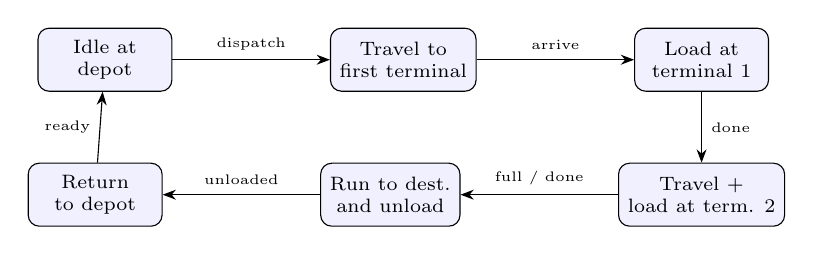
\begin{tikzpicture}[>=Stealth,node distance=2.0cm,
 st/.style={draw,rounded corners,minimum width=1.7cm,minimum height=0.8cm,align=center,font=\scriptsize,fill=blue!6}]
\node[st] (idle) {Idle at\\depot};
\node[st,right=of idle] (t1) {Travel to\\first terminal};
\node[st,right=of t1] (l1) {Load at\\terminal 1};
\node[st,below=0.9cm of l1] (l2) {Travel +\\load at term. 2};
\node[st,left=of l2] (dest) {Run to dest.\\and unload};
\node[st,left=of dest] (ret) {Return\\to depot};
\draw[->] (idle) -- node[above,font=\tiny]{dispatch} (t1);
\draw[->] (t1) -- node[above,font=\tiny]{arrive} (l1);
\draw[->] (l1) -- node[right,font=\tiny]{done} (l2);
\draw[->] (l2) -- node[above,font=\tiny]{full / done} (dest);
\draw[->] (dest) -- node[above,font=\tiny]{unloaded} (ret);
\draw[->] (ret) -- node[left,font=\tiny]{ready} (idle);
\end{tikzpicture}}
\caption{State-transition diagram of a bus (Point).}\label{fig:state}
\end{figure}

\begin{figure}[t]
\centering
\resizebox{0.95\columnwidth}{!}{%
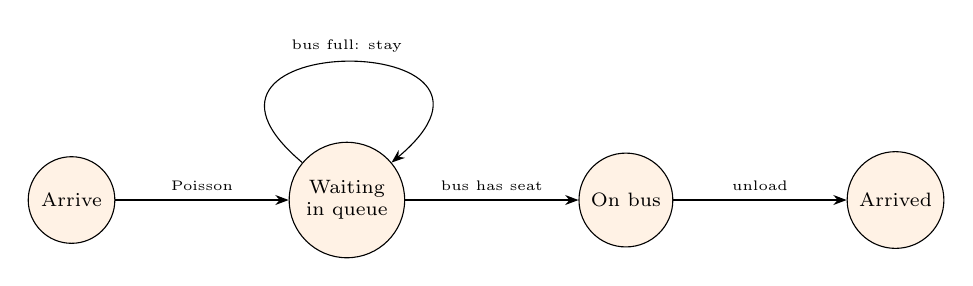
\begin{tikzpicture}[>=Stealth,node distance=2.2cm,
 st/.style={draw,circle,minimum size=1.1cm,align=center,font=\scriptsize,fill=orange!10}]
\node[st] (a) {Arrive};
\node[st,right=of a] (q) {Waiting\\in queue};
\node[st,right=of q] (b) {On bus};
\node[st,right=of b] (d) {Arrived};
\draw[->] (a) -- node[above,font=\tiny]{Poisson} (q);
\draw[->] (q) -- node[above,font=\tiny]{bus has seat} (b);
\draw[->] (b) -- node[above,font=\tiny]{unload} (d);
\draw[->] (q) to[out=140,in=40,looseness=6] node[above,font=\tiny]{bus full: stay} (q);
\end{tikzpicture}}
\caption{State-transition diagram of a passenger.}\label{fig:state2}
\end{figure}

\subsection{Flowchart of the simulation logic}
\begin{figure}[t]
\centering
\resizebox{0.9\columnwidth}{!}{%
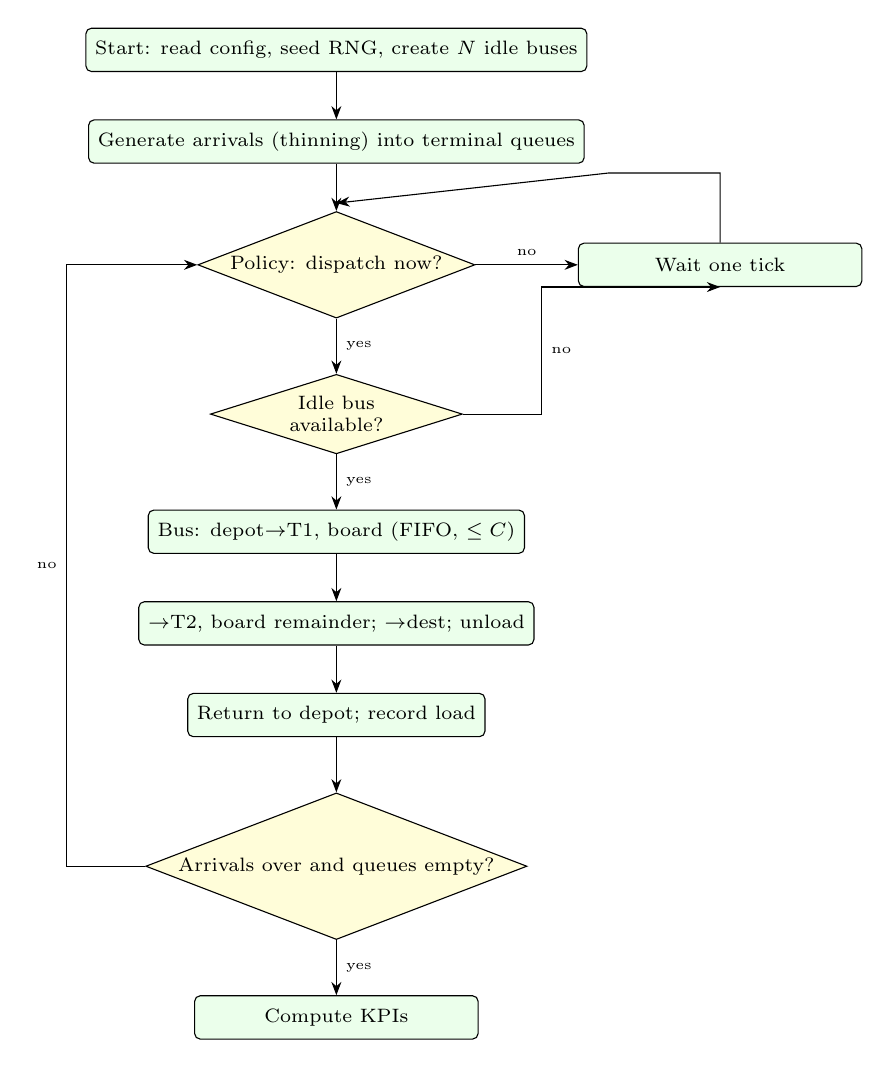
\begin{tikzpicture}[>=Stealth,node distance=0.6cm,
 p/.style={draw,rectangle,rounded corners=2pt,minimum width=3.6cm,minimum height=0.55cm,align=center,font=\scriptsize,fill=green!8},
 d/.style={draw,diamond,aspect=2.6,minimum width=3.2cm,align=center,font=\scriptsize,fill=yellow!15,inner sep=1pt}]
\node[p] (s) {Start: read config, seed RNG, create $N$ idle buses};
\node[p,below=of s] (arr) {Generate arrivals (thinning) into terminal queues};
\node[d,below=of arr] (pol) {Policy: dispatch now?};
\node[p,right=1.3cm of pol] (wait) {Wait one tick};
\node[d,below=0.7cm of pol] (bus) {Idle bus\\available?};
\node[p,below=0.7cm of bus] (go) {Bus: depot$\to$T1, board (FIFO, $\le C$)};
\node[p,below=of go] (go2) {$\to$T2, board remainder; $\to$dest; unload};
\node[p,below=of go2] (ret) {Return to depot; record load};
\node[d,below=0.7cm of ret] (end) {Arrivals over and queues empty?};
\node[p,below=0.7cm of end] (fin) {Compute KPIs};
\draw[->] (s)--(arr); \draw[->] (arr)--(pol);
\draw[->] (pol) -- node[above,font=\tiny]{no} (wait);
\draw[->] (wait) |- ($(arr.east)+(0.3,-0.4)$) -- ($(pol.north)+(0,0.1)$);
\draw[->] (pol) -- node[right,font=\tiny]{yes} (bus);
\draw[->] (bus.east) -- ++(1.0,0) |- node[near start,right,font=\tiny]{no} (wait.south);
\draw[->] (bus) -- node[right,font=\tiny]{yes} (go);
\draw[->] (go)--(go2); \draw[->] (go2)--(ret); \draw[->] (ret)--(end);
\draw[->] (end) -- node[right,font=\tiny]{yes} (fin);
\draw[->] (end.west) -- ++(-1.0,0) |- node[near start,left,font=\tiny]{no} (pol.west);
\end{tikzpicture}}
\caption{Flowchart of the discrete-event simulation.}\label{fig:flow}
\end{figure}

\section{Mathematical Model}
\subsection{Arrival process}
Arrivals at terminal $k\in\{1,2\}$ form a non-homogeneous Poisson process with intensity
\begin{equation}
\lambda_k(t)=\pi_k\Big[\lambda_0+\lambda_1\exp\!\Big(-\tfrac{(t-t_p)^2}{2s^2}\Big)\Big],
\end{equation}
where $\pi_k$ is the terminal share. Samples are drawn by Lewis--Shedler thinning: candidate events at the constant rate $\lambda^{\max}_k$, each accepted with probability $\lambda_k(t)/\lambda^{\max}_k$. The expected number of arrivals is $\int_0^{W}\!\sum_k\lambda_k(t)\,dt\approx 1147$ for $W=180$~min.

\subsection{Service capacity and bottleneck condition}
A bus completes one cycle in
\begin{equation}
T_c(t)=\kappa(t)\,(\ell_1+\ell_2+\ell_3+\ell_4)+2\delta+u+C\beta+4p_id_i,
\end{equation}
with leg times $\ell_j$, door dwell $\delta$, unloading $u$, per-passenger boarding time $\beta$ and congestion factor $\kappa(t)\in\{1,1.25\}$. A fleet of $N$ buses carrying full loads can therefore move at most
\begin{equation}
\mu(t)=\frac{N\,C}{T_c(t)}\quad\text{pax/min}.
\end{equation}
The system is a time-varying multi-server queue with bulk service, and the \emph{traffic intensity} is $\rho(t)=\lambda(t)/\mu(t)$. Whenever $\rho(t)>1$ the queue necessarily grows regardless of scheduling; scheduling can only (a) keep loads close to $C$, (b) keep buses evenly spaced and (c) share the capacity fairly between terminals. For the assumed parameters $\mu\approx 10.7$ pax/min in the peak against $\lambda_{\max}=14$, giving $\rho_{\max}=1.31$; $\rho>1$ between 08:12 and 08:48 (Fig.~\ref{fig:rho}).

\subsection{Performance measures}
For passenger $i$ boarding at time $b_i$ after arriving at $a_i$ the wait is $W_i=b_i-a_i$. We report the mean $\bar W$, median, 95th percentile $W_{95}$, maximum, peak queue $\max_t Q(t)$, the percentage of passengers who watch at least one full bus leave (``left behind''), average load factor $\bar\ell=\overline{\text{load}}/C$ and fleet utilisation (busy time over $N\times$ horizon). Little's law $\bar L=\lambda_{\text{eff}}\bar W$ is used as a check of the simulator.

\subsection{Dispatch policies}
\textbf{P0 Static (baseline).} A bus leaves every 5~min; if no bus is at the depot the slot is delayed and later slots bunch up.\par
\textbf{P1 Peak-aware timetable.} Headway $H(t)=\mathrm{clip}\!\big(0.9\,C/\lambda(t),\;4.2,\;5.0\big)$ min, computed from historical mean demand. The lower bound approximates $T_c/N\approx 4.7$~min, the spacing that the fleet can physically sustain.\par
\textbf{P2 Dynamic dispatch (reactive).} Dispatch when the \emph{net} queue (queue minus seats of buses already on their way) reaches 80\% of $C$, or reaches 40\% of $C$ with the oldest student waiting at least 5~min, or the oldest has waited 12~min (flush rule).\par
\textbf{P3 Hybrid adaptive.} Headway from a blend of the live EWMA arrival rate and the historical profile, $\hat\lambda=0.5\,\hat\lambda_{\text{EWMA}}+0.5\,\lambda_{\text{hist}}(t)$; buses never leave an empty system; the bus visits the terminal with the \emph{oldest} waiting student first and uses a fair-share seat quota $\max\{\lfloor C q_1/(q_1+q_2)\rceil,\,C-q_2\}$ at the first stop so that the second terminal is not starved.

\section{Simulation Implementation}
The simulator is written in Python~3 with SimPy~\cite{simpy}. The three processes below are the heart of the model; the complete source is in the GitHub repository.

\begin{lstlisting}
def arrivals_proc(self, k):      # NHPP by thinning
    lam_max = c.demand_scale*(c.base_rate+c.peak_rate)*c.share_terminal[k]
    t = 0.0
    while True:
        t += self.rng.exponential(1.0/lam_max)
        if t > c.window: return
        yield self.env.timeout(max(0.0, t - self.env.now))
        if self.rng.random() <= c.rate(t, k)/lam_max:
            self.queues[k].append([self.env.now, False])

def dispatcher_proc(self):
    while True:
        if self.policy.should_dispatch(self.env.now, self):
            bus = yield self.depot.get()   # blocks if fleet is out
            self.policy.on_dispatch(self.env.now, self)
            self.pending_seats += c.capacity
            self.env.process(self.bus_proc(bus, self.env.now))
        else:
            yield self.env.timeout(c.dispatch_tick)

def board(self, k, free):        # FCFS boarding
    while q and n < free:
        a, _ = q.popleft();  self.waits.append(self.env.now - a)
        n += 1
\end{lstlisting}

The dispatch rule of the best static policy is only a few lines:
\begin{lstlisting}
class StaticPeakAware(Policy):
    def headway_at(self, t):
        lam = self.cfg.total_rate(min(t, self.cfg.window))
        return clip(0.9*self.cfg.capacity/lam, 4.2, 5.0)
    def should_dispatch(self, t, sys): return t >= self.next_slot
    def on_dispatch(self, t, sys):
        self.next_slot += self.headway_at(self.next_slot)
\end{lstlisting}

\section{Experimental Design, Verification and Validation}
\textbf{Replications.} Each policy is run 50 times (seeds 0--49) for each scenario; tables report means with 95\% confidence half-widths $1.96\,s/\sqrt{n}$ and Welch $t$-tests. Policy parameters were tuned on a \emph{separate} seed set (1000+) so the reported numbers are not over-fitted to the evaluation seeds.

\textbf{Verification} (\texttt{tests/verify.py}, all pass): (1) every arrival is served for all four policies; (2) simulated mean arrivals 1150.1 against the analytic 1146.6 (0.3\% error); (3) a deterministic single-passenger run waits 5.5~min, matching the first leg; (4) bus load never exceeds $C$; (5) Little's law: $\int Q\,dt=8647$ versus $\sum W_i=8621$ pax-min (0.3\%); (6) mean wait increases monotonically with demand (4.4, 7.9, 13.6~min at 80, 100, 120\%).

\textbf{Validation.} The analytic bottleneck window ($\rho>1$, 08:12--08:48) coincides with the onset of queue growth in the simulated baseline (Fig.~\ref{fig:queue}), and the baseline reproduces the qualitative symptoms of the brief (long peak queues, over-capacity buses, uneven terminals). Quantitative validation against real counts is not possible without field data; see Section~\ref{sec:limits}.

\section{Results}
\subsection{Baseline bottleneck analysis}
Figure~\ref{fig:rho} shows demand against fleet capacity. The fleet cannot carry the peak: for about 36 minutes $\rho>1$ and the baseline queue grows to a mean peak of 180 students (Fig.~\ref{fig:queue}). The baseline also shows a structural bias: because every bus visits STC first, STC students wait 3.2~min on average whereas Main Gate students wait 13.4~min (Fig.~\ref{fig:fair}). In the baseline 28\% of students watch at least one full bus leave and the average load is 73\% of capacity (full at the peak, 14--26 passengers off-peak).

\begin{figure}[t]\centering
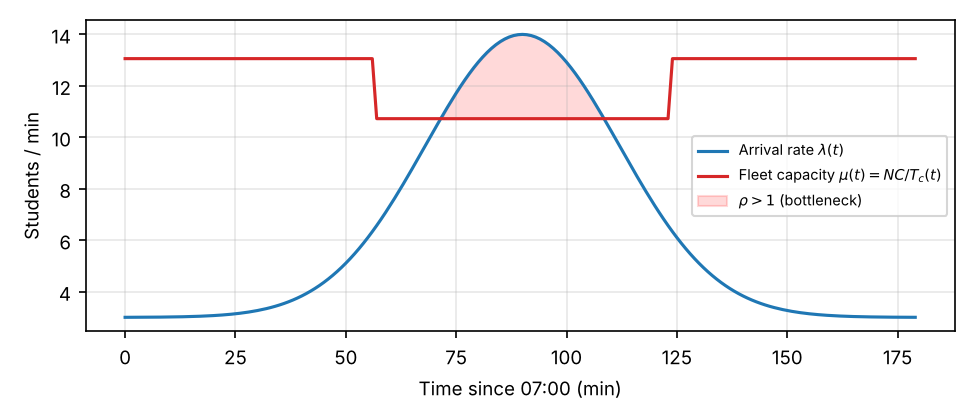
\includegraphics[width=\columnwidth]{figures/rho_curve.png}
\caption{Arrival rate versus fleet capacity; the shaded region is the bottleneck ($\rho>1$).}\label{fig:rho}
\end{figure}

\subsection{Policy comparison (morning session)}
\begin{table*}[t]
\centering\caption{Morning session, 12 buses, 50 replications (mean $\pm$ 95\% CI)}\label{tab:main}
\begin{tabular}{@{}lccccccc@{}}
\toprule
Policy & Mean wait & 95th pct & Max wait & Peak queue & Fleet util. & Left behind & Wait STC / MG\\
 & (min) & (min) & (min) & (students) & & (\%) & (min)\\
\midrule
P0 Static (baseline) & $7.75\pm0.26$ & $27.7\pm1.0$ & $32.8\pm1.1$ & $180\pm6$ & $0.63$ & $28.5$ & $3.2$ / $13.4$\\
P1 Peak-aware timetable & $\mathbf{6.09\pm0.23}$ & $19.0\pm1.1$ & $25.2\pm1.3$ & $\mathbf{148\pm7}$ & $\mathbf{0.67}$ & $\mathbf{26.3}$ & $3.2$ / $9.7$\\
P2 Dynamic dispatch & $12.60\pm0.24$ & $32.2\pm1.0$ & $37.8\pm1.1$ & $231\pm5$ & $0.47$ & $41.6$ & $5.4$ / $21.6$\\
P3 Hybrid adaptive & $8.63\pm0.33$ & $\mathbf{18.0\pm0.7}$ & $\mathbf{22.6\pm0.9}$ & $177\pm6$ & $0.64$ & $58.2$ & $\mathbf{8.6}$ / $\mathbf{8.7}$\\
\bottomrule
\end{tabular}
\end{table*}

Table~\ref{tab:main} and Figs.~\ref{fig:queue}--\ref{fig:cdf} summarise the comparison. Relative to P0:
\begin{itemize}
\item \textbf{P1} lowers the mean wait by 21.4\% and the 95th percentile by 31.1\% ($p<10^{-14}$ in both cases) and cuts the peak queue by 18\%, with the same fleet. It improves every waiting and queue metric.
\item \textbf{P3} gives the lowest tail (95th percentile $-34.8\%$, maximum wait $-31\%$) and removes the terminal inequity (8.6 vs 8.7~min), but its mean is 11\% \emph{higher} than the baseline: serving the longer queue first (as the baseline implicitly does) minimises the mean, whereas the fair-share quota trades mean for equity. P3 also leaves more students behind (58\%) because the quota splits seats between the two terminals.
\item \textbf{P2} is clearly worse (mean $+63\%$). A purely reactive rule waits for the queue to reach a threshold, which adds accumulation delay off-peak (median 8.9 versus 4.1~min), and fleet utilisation drops to 47\% because buses sit at the depot until the threshold is met. Seat load factor is very high (98\%) yet waiting is longer: full buses are not the same as short waits.
\end{itemize}

\begin{figure}[t]\centering
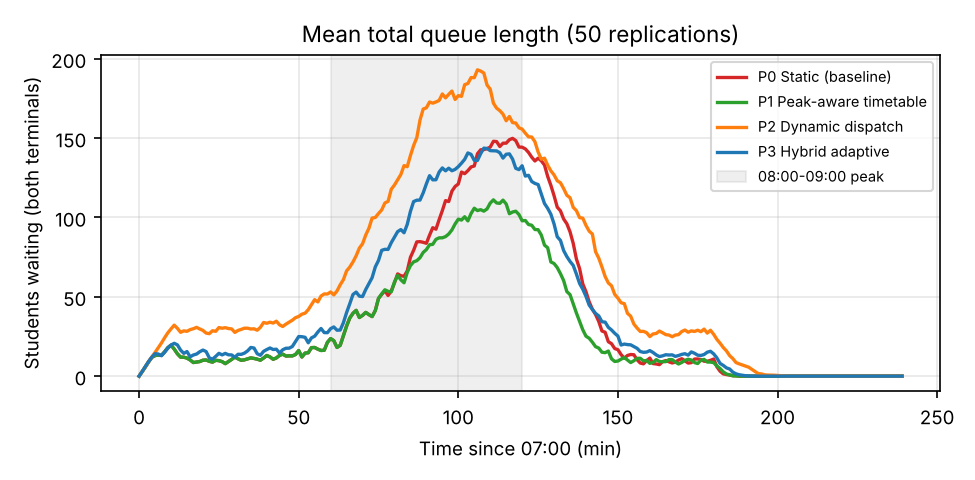
\includegraphics[width=\columnwidth]{figures/queue_over_time.png}
\caption{Mean total queue over time for the four policies.}\label{fig:queue}
\end{figure}
\begin{figure}[t]\centering
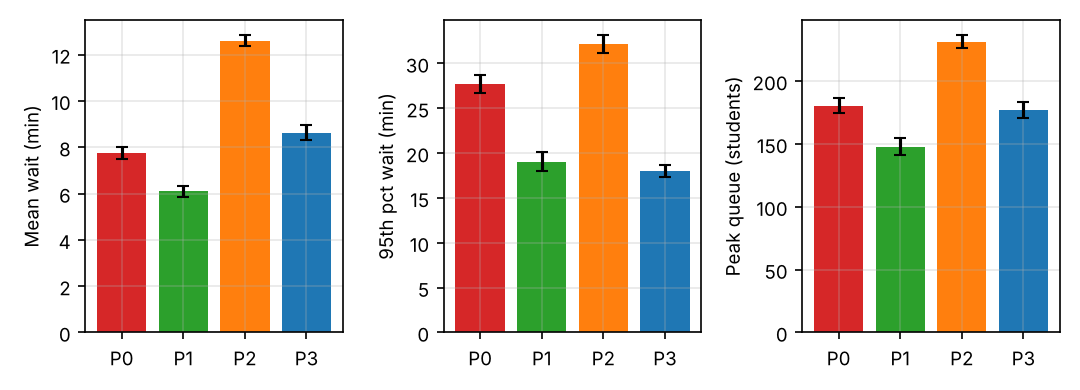
\includegraphics[width=\columnwidth]{figures/metric_bars.png}
\caption{Mean wait, 95th percentile wait and peak queue (error bars: 95\% CI).}\label{fig:bars}
\end{figure}
\begin{figure}[t]\centering
\begin{minipage}{0.49\columnwidth}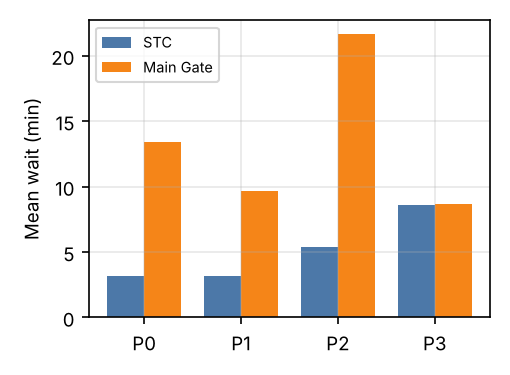
\includegraphics[width=\linewidth]{figures/terminal_fairness.png}\end{minipage}
\begin{minipage}{0.49\columnwidth}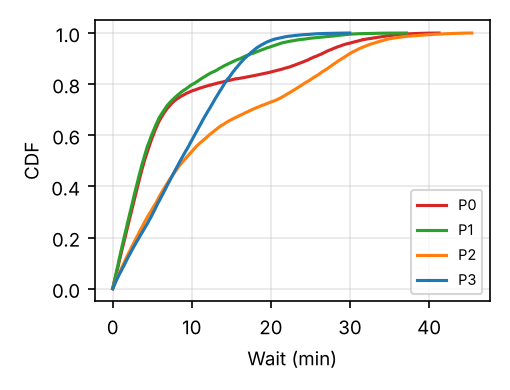
\includegraphics[width=\linewidth]{figures/wait_cdf.png}\end{minipage}
\caption{Left: mean wait by terminal. Right: empirical CDF of student waits.}\label{fig:fair}\label{fig:cdf}
\end{figure}

\subsection{What-if analysis}
\textbf{Fleet size (Fig.~\ref{fig:fleet}).} With the baseline schedule, 12 buses give a mean wait of 7.8~min; under P1 \emph{11} buses give 7.3~min and a better 95th percentile (24.9 vs 27.4~min), i.e.\ scheduling is worth about one bus. Beyond 13 buses nothing improves because the headway bounds (4.2--5~min) rather than the fleet become the limit; at 8--9 buses all policies degrade sharply and P1 coincides with P0 because the fleet itself is the bottleneck. P3 keeps a lower tail than P0 at every fleet size from 8 to 12.

\textbf{Demand surge (Fig.~\ref{fig:demand}).} P1 dominates P0 from 80\% to 130\% of baseline demand (e.g.\ at 130\% the mean is 12.3 vs 16.3~min). P3's tail advantage grows with load (95th percentile 33.7 vs 52.9~min at 130\%) and its mean converges to P0's at 120\% and above. P2 has the highest mean at every demand level and approaches P0 only under heavy overload.

\textbf{Traffic uncertainty.} Raising the travel noise from $\sigma=0.10$ with 1\% incidents to $\sigma=0.40$ with 10\% incidents increases the P0 mean from 7.0 to 9.4~min; P1 stays 1.3--1.7~min better throughout, and the tail advantage of P3 stays at 8--10~min. \textbf{Afternoon session.} The ranking is the same: P1 reduces the mean wait from 7.3 to 5.9~min and the 95th percentile from 23.0 to 16.2~min; P3 reaches 17.0~min with equal terminal waits.

\textbf{Ablation.} Removing the adaptive stop order from P3 gives P1-like behaviour (mean 6.5, STC/MG 3.2/10.5~min); adding express (single-stop) trips with an assumed 4-minute saving gave no meaningful gain (mean 8.5 vs 8.7~min) and a slightly worse tail (95th percentile 19.3 vs 18.0~min), so it is not recommended under these assumptions.

\begin{figure}[t]\centering
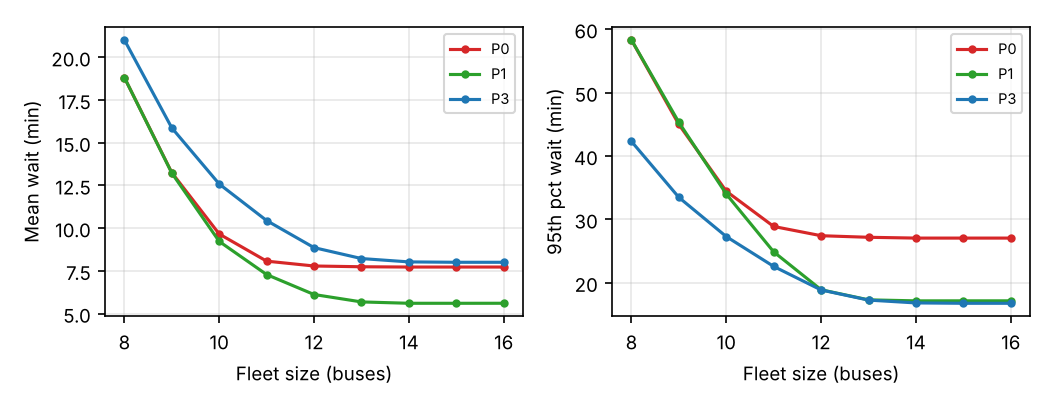
\includegraphics[width=\columnwidth]{figures/fleet_sweep.png}
\caption{Effect of fleet size on mean and 95th percentile wait.}\label{fig:fleet}
\end{figure}
\begin{figure}[t]\centering
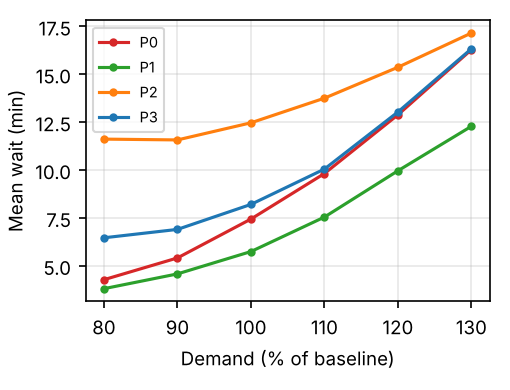
\includegraphics[width=0.75\columnwidth]{figures/demand_scenarios.png}
\caption{Mean wait versus demand level.}\label{fig:demand}
\end{figure}

\section{Recommendations}
\begin{enumerate}
\item \textbf{Adopt a demand-shaped timetable (P1)} with 4.5-minute headway in the 08:00--09:00 and 14:00--15:30 peaks and 5-minute headway otherwise. It needs no technology, only a revised timetable, and gave $-21\%$ mean and $-31\%$ 95th-percentile waiting. It is equivalent to adding about one bus.
\item \textbf{Fix the terminal imbalance.} Rotate the first stop between STC and Main Gate, or reserve a seat quota for the second terminal. If equity of waiting time and a short tail matter more than the mean (P3), use the fair-share quota, which brings the 95th percentile down by 35\% and equalises STC and Main Gate.
\item \textbf{Do not use a purely reactive ``leave when full'' rule}; it increased the mean wait by 63\% in the baseline scenario and was worse than the static baseline at every demand level tested. Live data should be used to \emph{regulate headways}, not to hold buses.
\item \textbf{Manage the 08:12--08:48 window explicitly.} Demand exceeds fleet capacity by up to 31\%; the only remaining levers are shifting classes by 15--20 minutes, adding short-haul express services, or one extra bus. The what-if analysis shows each is worth testing before spending.
\item \textbf{Collect data} (stop-level counts, GPS) to calibrate and then re-run the supplied simulator; changing \texttt{config.py} is enough.
\end{enumerate}

\section{Limitations and Threats to Validity}\label{sec:limits}
All demand and travel-time parameters are assumptions; absolute waits will differ at MUET and the policy ranking should be re-checked after calibration. The model has two terminals and one corridor, ignores multiple routes, driver breaks, breakdowns and student reneging, assumes the same capacity for every bus and models traffic as log-normal noise plus incidents. Policy parameters were tuned by grid search on one scenario; they are tuned, not proven optimal. The express-trip saving (4 min) is assumed. Finally, P3's fairness gain is measured on waiting time only; it does not reflect student preference for shorter versus more equal waits.

\section{Conclusion}
Modeling the MUET Point system as a time-varying queue shows that the morning peak exceeds fleet capacity by up to 31\% for about 36 minutes, which no schedule can fully remove, but that scheduling still matters: a demand-shaped timetable cut mean waiting by 21\% and the 95th percentile by 31\% with no new buses, a fair-share hybrid cut the tail by 35\% and equalised the two terminals, and a reactive policy did worse than the status quo. The simulator, configuration and experiments are reproducible and ready to be calibrated with real MUET data.

\begin{thebibliography}{9}
\bibitem{law} A.~M. Law, \emph{Simulation Modeling and Analysis}, 5th ed. New York: McGraw-Hill, 2015.
\bibitem{banks} J.~Banks, J.~S. Carson, B.~L. Nelson and D.~M. Nicol, \emph{Discrete-Event System Simulation}, 5th ed. Upper Saddle River, NJ: Pearson, 2010.
\bibitem{simpy} SimPy Developers, ``SimPy: Discrete event simulation for Python,'' \url{https://simpy.readthedocs.io}.
\bibitem{lewis} P.~A.~W. Lewis and G.~S. Shedler, ``Simulation of nonhomogeneous Poisson processes by thinning,'' \emph{Naval Research Logistics Quarterly}, vol.~26, no.~3, pp.~403--413, 1979.
\bibitem{little} J.~D.~C. Little, ``A proof for the queuing formula: $L=\lambda W$,'' \emph{Operations Research}, vol.~9, no.~3, pp.~383--387, 1961.
\bibitem{vuchic} V.~R. Vuchic, \emph{Urban Transit: Operations, Planning and Economics}. Hoboken, NJ: Wiley, 2005.
\end{thebibliography}
\end{document}
